\section{Benchmark}

All benchmarks were compiled using \texttt{g++} 13.3.0 and executed on an Intel Core i5 2.60\,GHz CPU. One of the test sets uses data from the US Road System, available at \url{https://www.diag.uniroma1.it/~challenge9/download.shtml}.

\subsection{Performance Evaluation}

To assess the performance of the various priority queues, several scenarios were considered:

\begin{itemize}
  \item \textbf{Universe size scaling:} Time and memory usage were measured for different integer key universe sizes, using 1,000,000 randomized \texttt{push} and \texttt{pop} operations. This test was designed to evaluate how integer-based priority queues scale with increasing key space.

  \item \textbf{Queue size scaling:} To examine the effect of queue size, a fixed universe size of $2^{25}$ was used. For each test, a bulk of elements was inserted using \texttt{push} operations, followed by their removal using \texttt{pop}. Time and memory usage were measured separately for both phases.

  \item \textbf{String key performance:} (General-purpose queues only) This test assessed time usage when operating on long random string keys (1024 characters), with varying queue sizes. The goal was to evaluate the impact of costly key comparisons on overall performance.

  \item \textbf{Practical application:} (General-purpose queues only) Each queue was integrated into Dijkstra's shortest path algorithm and tested on real-world graphs from the 9th DIMACS Implementation Challenge. Datasets of various sizes from the US Road System were used to compare real-world runtime performance.
\end{itemize}

Below we provide results of the performance test scenarios mentioned. In many cases we also provide a baseline implementation from the C++ STL Library for comparison:

\begin{figure}[H]
    \centering
    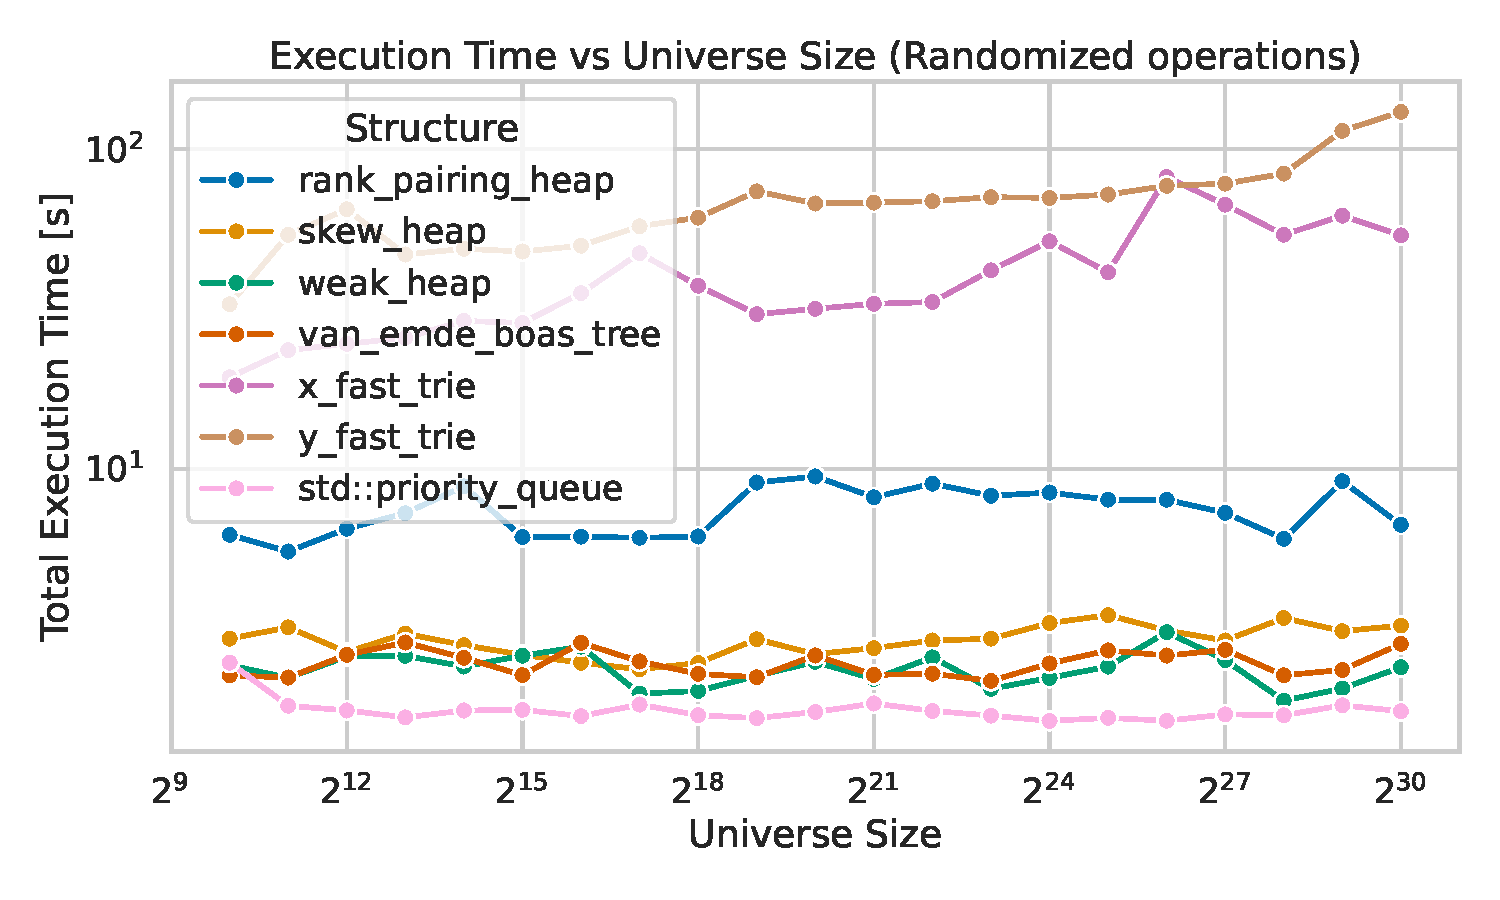
\includegraphics[width=1.0\textwidth]{figures/plots/plot_universe_vs_time.pdf}
    \caption{Total execution time vs. universe size.}
    \label{fig:execution_time}
\end{figure}

\begin{figure}[H]
    \centering
    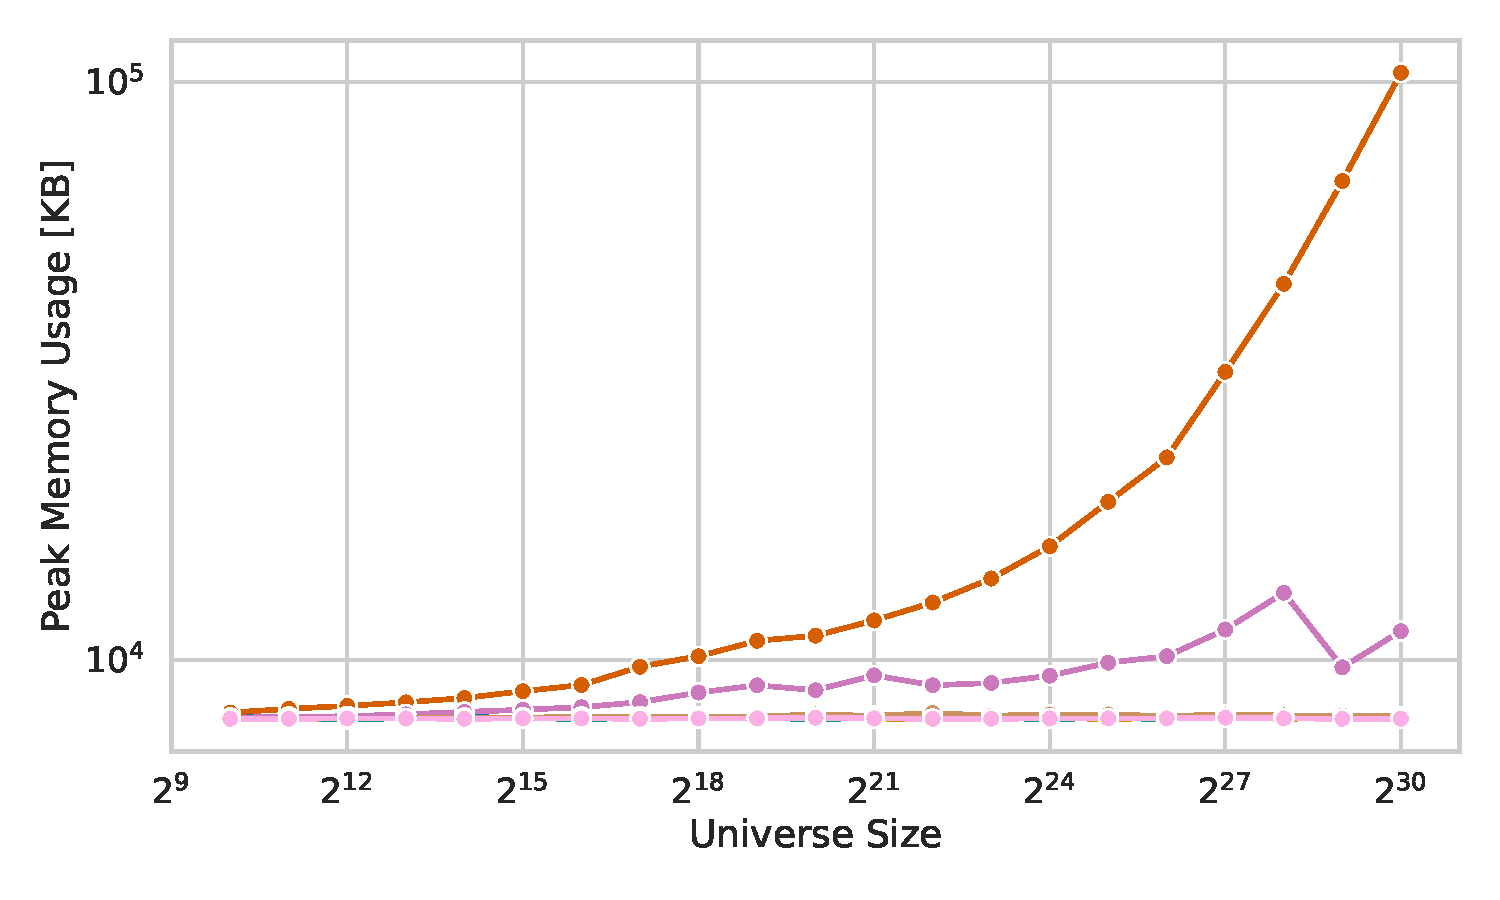
\includegraphics[width=1.0\textwidth]{figures/plots/plot_universe_vs_memory.pdf}
    \caption{Memory usage vs. universe size.}
    \label{fig:execution_time}
\end{figure}

\begin{figure}[H]
    \centering
    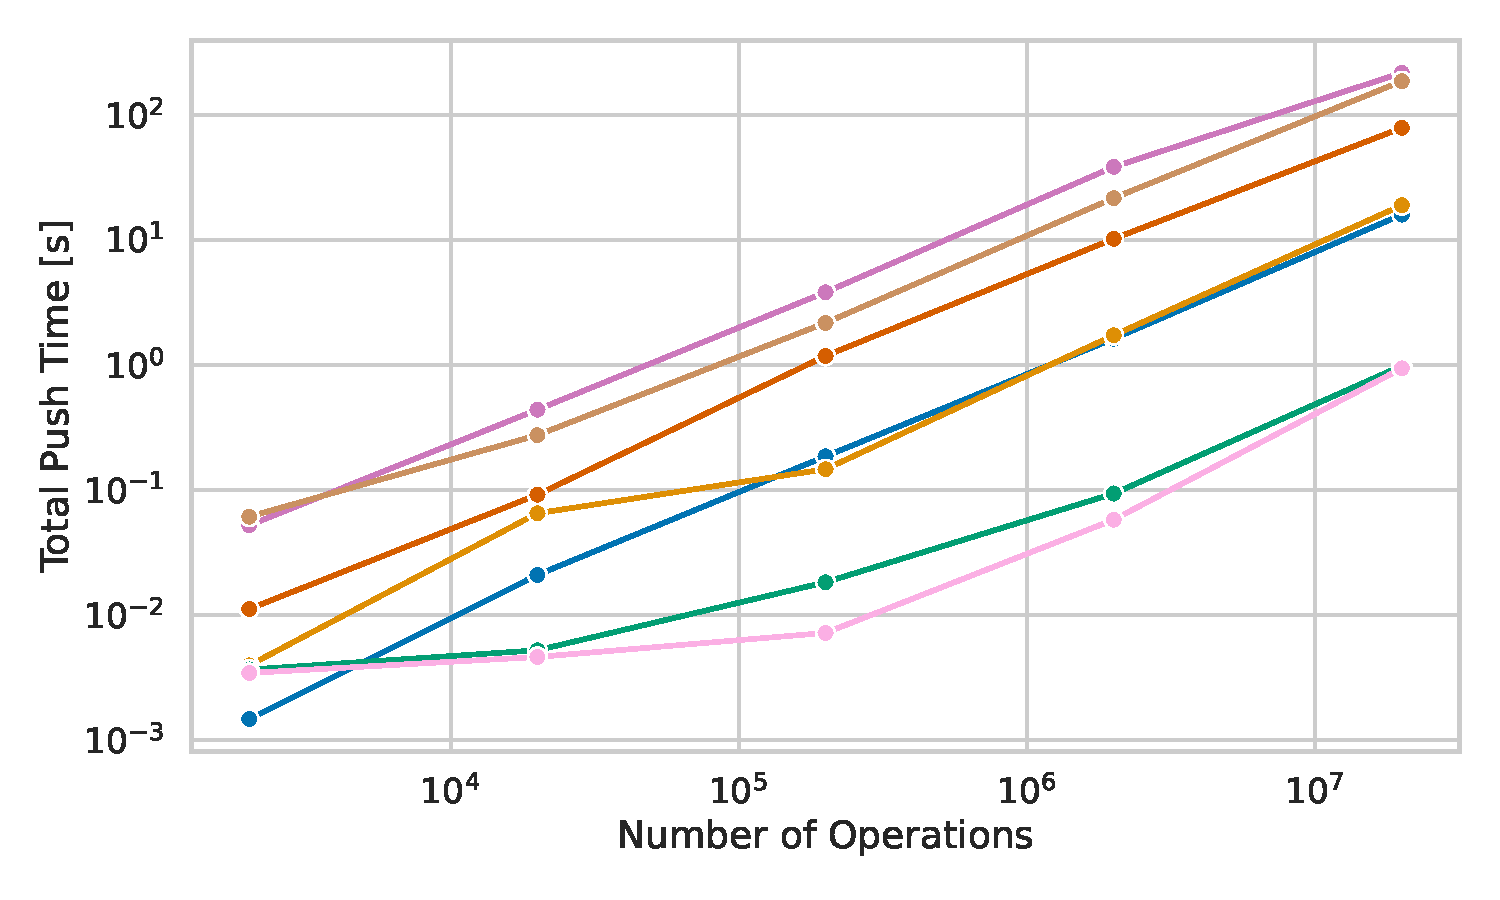
\includegraphics[width=1.0\textwidth]{figures/plots/plot_bulk_push.pdf}
    \caption{Push execution time vs. number of operations.}
    \label{fig:execution_time}
\end{figure}

\begin{figure}[H]
    \centering
    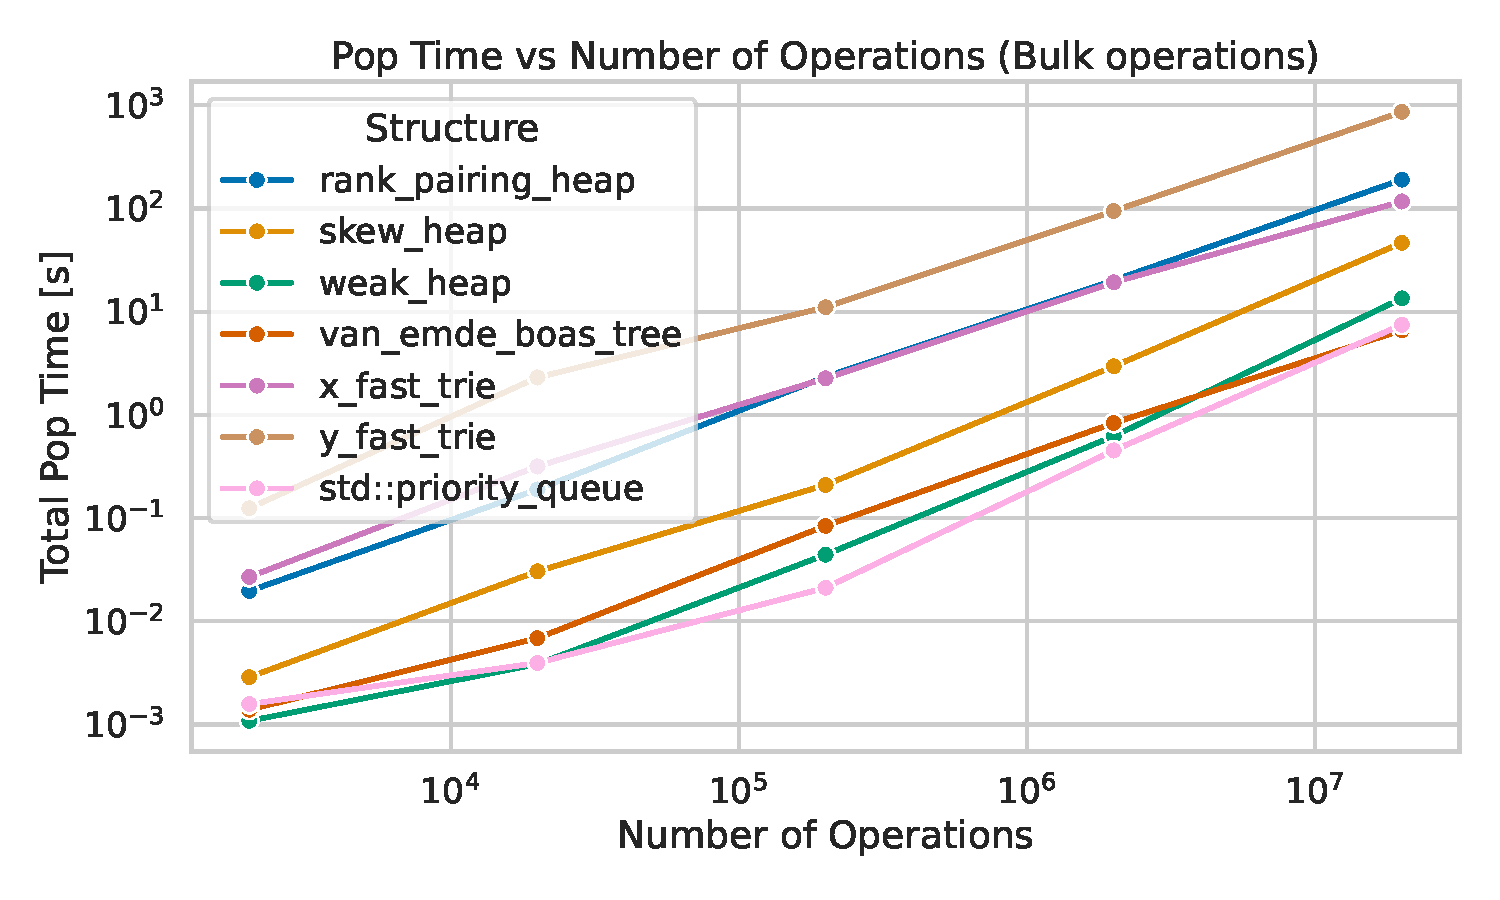
\includegraphics[width=1.0\textwidth]{figures/plots/plot_bulk_pop.pdf}
    \caption{Pop execution time vs. number of operations.}
    \label{fig:execution_time}
\end{figure}

\begin{figure}[H]
    \centering
    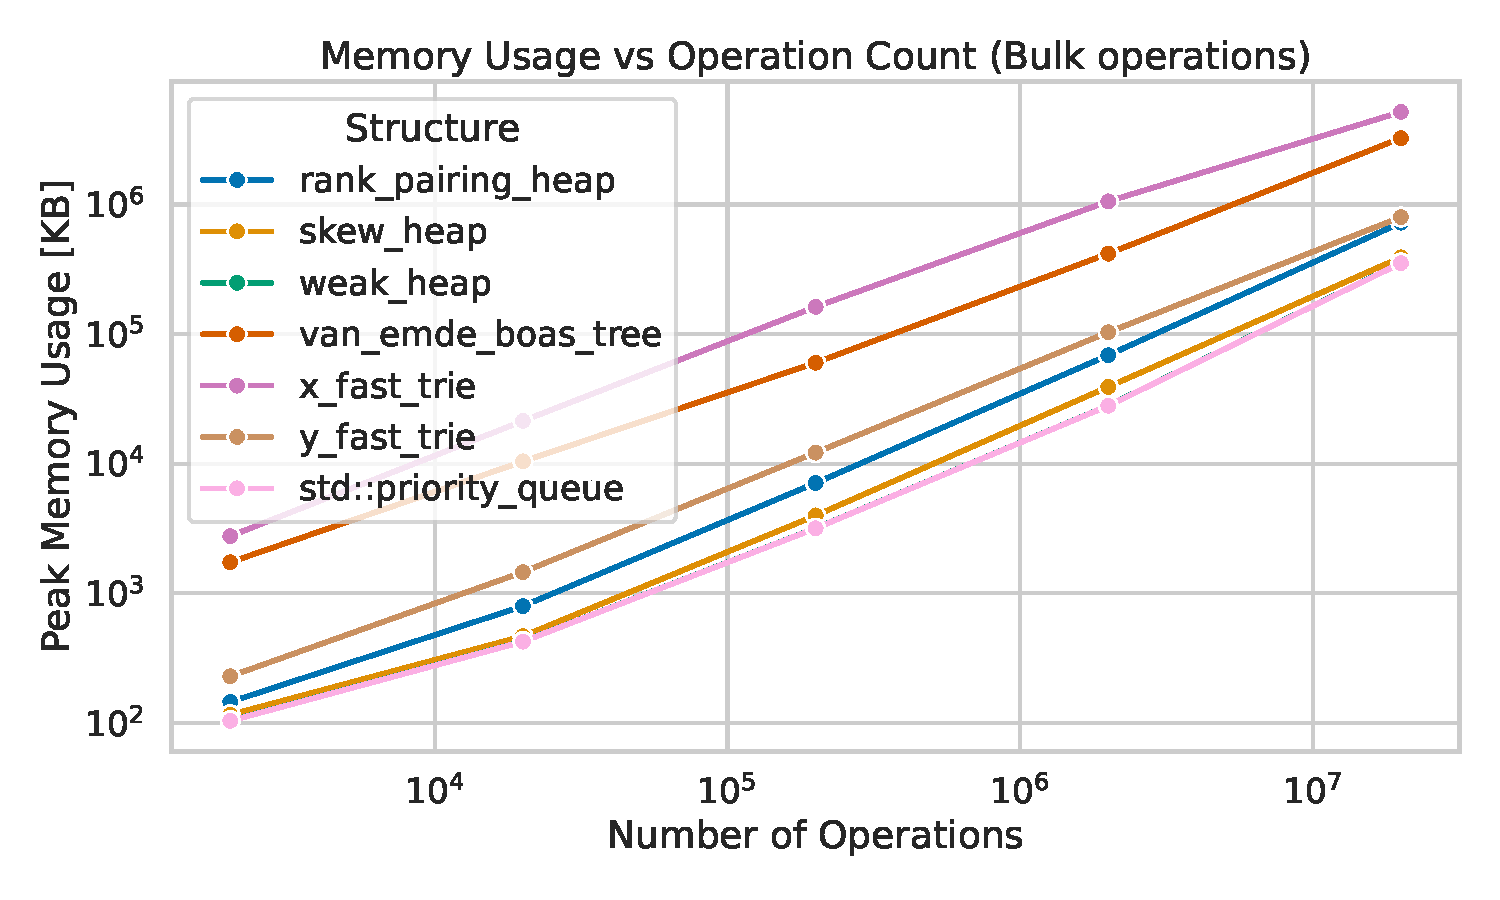
\includegraphics[width=1.0\textwidth]{figures/plots/plot_bulk_memory.pdf}
    \caption{Memory usage vs. number of operations.}
    \label{fig:execution_time}
\end{figure}

\begin{figure}[H]
    \centering
    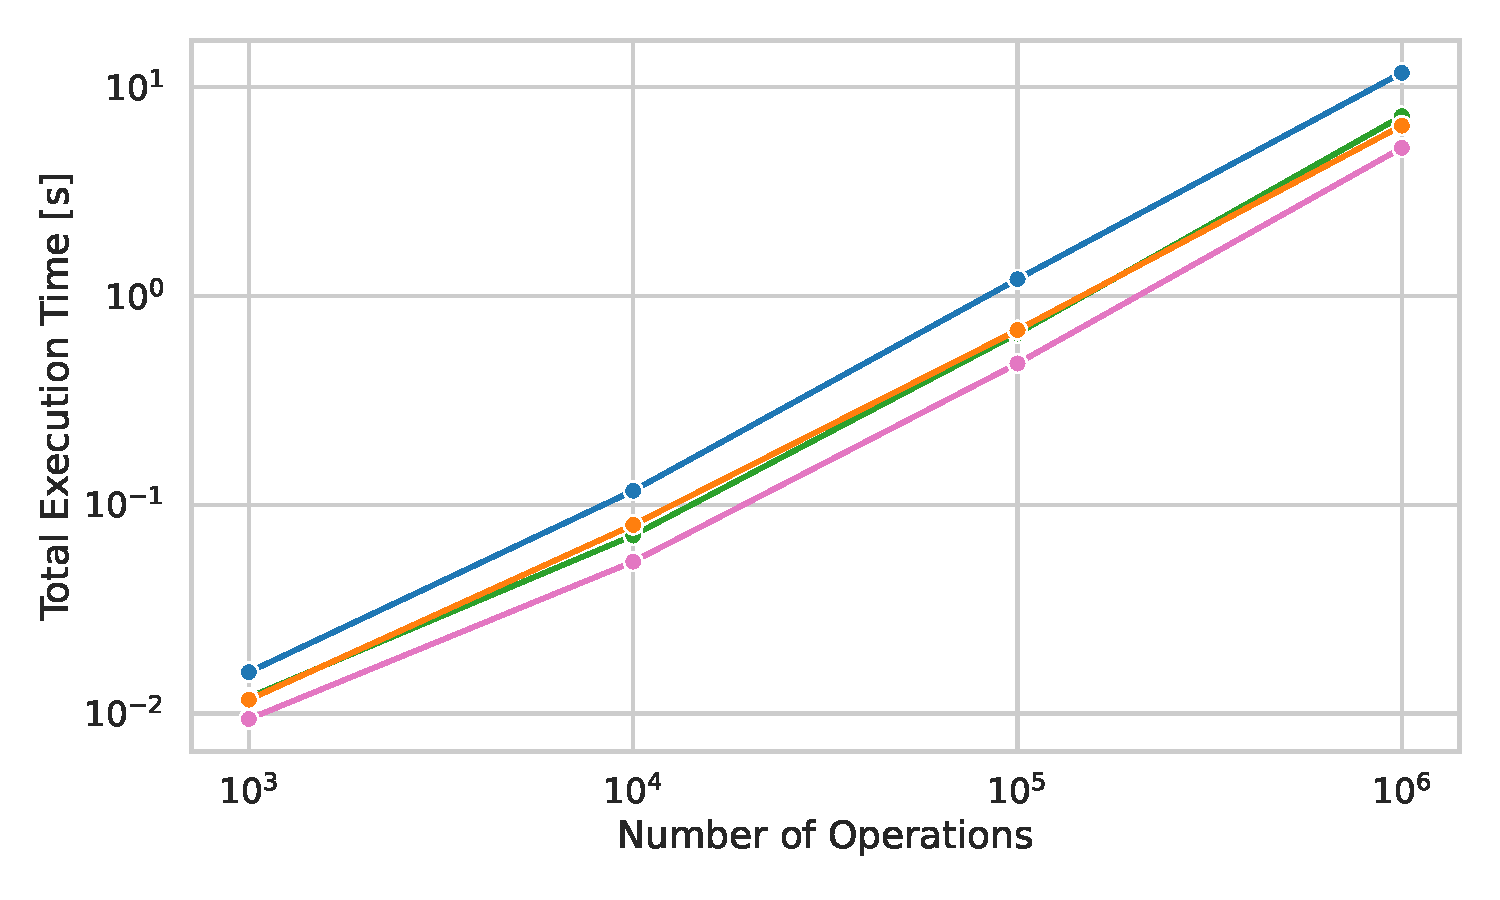
\includegraphics[width=1.0\textwidth]{figures/plots/plot_string_performance.pdf}
    \caption{Total execution time vs number of operations on string keys.}
    \label{fig:execution_time}
\end{figure}

\begin{table}[ht]
\centering
\begin{tabular}{|l|l|r|r|r|r|}
\hline
\textbf{Queue} & \textbf{File} & \textbf{Nodes} & \textbf{Edges} & \textbf{File Size} & \textbf{Time (s)} \\
\hline
weak\_heap         & USA-road-d.NY.gr   & 264,346    & 730,100     & 13.77 MB  & 0.0578 \\
skew\_heap         & USA-road-d.NY.gr   & 264,346    & 730,100     & 13.77 MB  & 0.0323 \\
rank\_pairing\_heap & USA-road-d.NY.gr   & 264,346    & 730,100     & 13.77 MB  & 0.1410 \\
std::priority\_queue & USA-road-d.NY.gr  & 264,346    & 730,100     & 13.77 MB  & 0.0335 \\
\hline
weak\_heap         & USA-road-d.FLA.gr  & 1,070,376  & 2,687,902   & 53.07 MB  & 0.2369 \\
skew\_heap         & USA-road-d.FLA.gr  & 1,070,376  & 2,687,902   & 53.07 MB  & 0.1402 \\
rank\_pairing\_heap & USA-road-d.FLA.gr  & 1,070,376  & 2,687,902   & 53.07 MB  & 0.5291 \\
std::priority\_queue & USA-road-d.FLA.gr & 1,070,376  & 2,687,902   & 53.07 MB  & 0.1427 \\
\hline
weak\_heap         & USA-road-d.CAL.gr  & 1,890,815  & 4,630,444   & 95.41 MB  & 0.4981 \\
skew\_heap         & USA-road-d.CAL.gr  & 1,890,815  & 4,630,444   & 95.41 MB  & 0.2951 \\
rank\_pairing\_heap & USA-road-d.CAL.gr  & 1,890,815  & 4,630,444   & 95.41 MB  & 0.9647 \\
std::priority\_queue & USA-road-d.CAL.gr & 1,890,815  & 4,630,444   & 95.41 MB  & 0.3153 \\
\hline
weak\_heap         & USA-road-d.W.gr    & 6,262,104  & 15,119,284  & 325.84 MB & 1.6977 \\
skew\_heap         & USA-road-d.W.gr    & 6,262,104  & 15,119,284  & 325.84 MB & 1.0162 \\
rank\_pairing\_heap & USA-road-d.W.gr    & 6,262,104  & 15,119,284  & 325.84 MB & 3.2455 \\
std::priority\_queue & USA-road-d.W.gr   & 6,262,104  & 15,119,284  & 325.84 MB & 1.1301 \\
\hline
weak\_heap         & USA-road-d.CTR.gr  & 14,081,816 & 33,866,826  & 756.36 MB & 5.7985 \\
skew\_heap         & USA-road-d.CTR.gr  & 14,081,816 & 33,866,826  & 756.36 MB & 4.5255 \\
rank\_pairing\_heap & USA-road-d.CTR.gr  & 14,081,816 & 33,866,826  & 756.36 MB & 10.0441 \\
std::priority\_queue & USA-road-d.CTR.gr & 14,081,816 & 33,866,826  & 756.36 MB & 4.3664 \\
\hline
weak\_heap         & USA-road-d.USA.gr  & 23,947,347 & 57,708,624  & 1322.82 MB& 7.0490 \\
skew\_heap         & USA-road-d.USA.gr  & 23,947,347 & 57,708,624  & 1322.82 MB& 4.3979 \\
rank\_pairing\_heap & USA-road-d.USA.gr  & 23,947,347 & 57,708,624  & 1322.82 MB& 13.3550 \\
std::priority\_queue & USA-road-d.USA.gr & 23,947,347 & 57,708,624  & 1322.82 MB& 4.6924 \\
\hline
\end{tabular}
\caption{Benchmark results for general-purpose priority queues, running the Dijkstra's algorithm on USA road network graphs.}
\end{table}